\chapter{Freight Traffic}
\label{ch:freight}
% ##################################################################################################################

\hfill \textbf{Authors:} Michael Zilske, Johan W. Joubert

\begin{center} 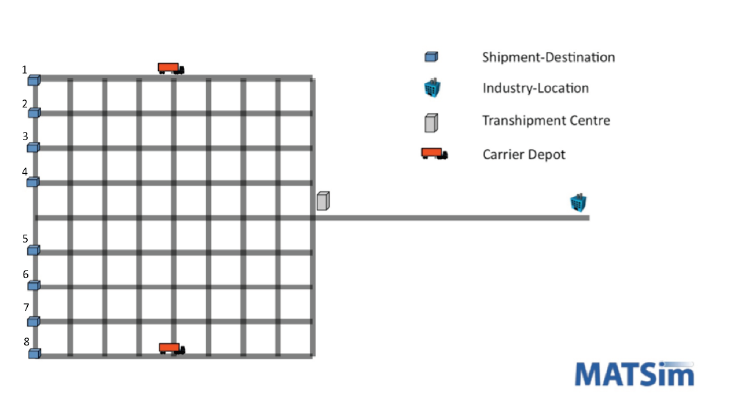
\includegraphics[width=0.65\textwidth, angle=0]{extending/figures/freightcarriers} \end{center}

\editdone{This text has undergone the professional edit. Please no grammatical changes anymore! They are most-probably wrong.}

\createStandardInformation{freight}{\lstinline|RunChessboard| class}{freight}{\citet[][]{SchroederZilskeEtAl2011TransportServiceProvider,ZilskeEtc2012AddingFreightToMatsim}}

% ##################################################################################################################
Various \gls{matsim} freight traffic modeling approaches have been implemented in recent years. 

For Zürich, available origin-destination matrices for small delivery trucks and heavy trucks have been disaggregated \citet[][]{ShahM_TechRep_IVT_2010}. Data was taken from the \gls{kvmzh} provided by \citet{AMV_Webpage_2011} and documented in \citet[][]{GottardiBuergler_SV_1999}. This special freight sub-population is restricted to route choice.

In South Africa, freight vehicles' plans were derived from \gls{gps} records of more than 30\,000 commercial vehicles tracked over a 6-month period.  Activity chains' extraction from raw \gls{gps} data was documented in \citet[][]{JoubertAxhausen_JTG_2011}; the first joint private car and freight implementation appeared in \citet[][]{JoubertJEtAl_TRR_2010}. In \citet[][]{NagelKickhoeferJoubert2014HeterogeneousVoTsPROCEDIA}, we used \gls{matsim} to evaluate the impact of a complex vehicle-type specific toll structure where sub-populations, including freight, have different time values.

The most sophisticated solution, however, was the introduction of carrier agents, described in the following section. 

% ##################################################################################################################
\section{Carriers}
\label{sec:carriers}
Until now, real-world scenarios set up with \gls{matsim} modeled freight traffic demand share by using plan sets with activities at the depot and pick-up and delivery locations, without variability in any dimension except route choice. We improved this situation by modeling freight vehicles as non-autonomous agents employed by, and serving the interests of, freight operators. Freight vehicle drivers' missing choice dimensions are then realized as logistics decisions made by the freight operators who employ them. In the freight transport sector, decisions are distributed among actors with different roles. Freight transport decisions include: lot-size choice, path-searches in logistical networks, vehicle choice and tour planning. A freight operator's planning problem is quite different from its passenger counterpart.

First, success of freight transport plans is not determined by the utility of time
spent at activity locations, but rather by commercial success. Plans must fulfill
customers' requirements, \ie time windows and providing sufficient capacity at
reasonable cost.

Second, freight operators often operate several vehicles and their
options include rescheduling deliveries from one vehicle to another or even changing the
number of vehicles used .

Thus, a new software layer populated by \emph{carrier agents} was introduced into the
simulation. Each carrier agent represents a firm with a vehicle fleet, depots and contracts.
Contracts determine type and quantity of goods to be carried and contains the respective 
origin and destination as well as pick-up and delivery time windows.

The carrier agent's plan contains a tour schedule  for each fleet  vehicle, containing 
planned pick-up, delivery or arrival times at customer locations and a route through 
the physical network. In our basic model, all vehicle schedules of a carrier begin and end at one of its depots.
When a simulation scenario is initialized, the carrier agents build a schedule for each of their vehicles, 
including a route through the transport network, with pick-up and delivery activities corresponding to their contracts.
At the interface between the freight operator plans and the mobility simulation, the set of routed vehicles 
from each carrier plan is injected into the traffic demand as individual driver agents, where they move 
through the traffic system along with passenger vehicles. While executing their plans, the freight driver 
agents report their shipment-related activities back to the carrier.

When all plans have been executed, agents evaluate the success of their plan. The carrier agents use a custom 
utility function capturing their economic success. Their cost is calculated as a sum of vehicle-dependent 
distance and time costs incurred by scheduled vehicles, as well as some individual fixed costs, plus penalties 
incurred by missed time windows.

Finally, carrier agents create new plans to improve their performance in the next iteration. For instance, a time-dependent vehicle routing heuristic can be plugged in to replan vehicle schedules. Shipments can be switched between vehicles, or an entire vehicle added or removed.
During repeated executions of their plans, passengers as well as carriers gain experience from the transport system. The carriers experience congestion and other disturbances in the traffic system when they incur a higher cost through longer vehicle usage, or by penalizing missed pick-up and delivery times.

The planning algorithms themselves are implemented in the project \lstinline|jsprit|, a library separate from \gls{matsim}.
In the replanning phase of each iteration, \lstinline|jsprit| is called and replans the carrier plans.

The model is described in a paper by \citet[][]{SchroederZilskeEtAl2011TransportServiceProvider}. For more details about the implementation, as well as more references, see the technical report by \citet[][]{ZilskeEtc2012AddingFreightToMatsim}.

% Package that plugs freight algorithms (programmed in external package jsprit) into matsim.
% * A good starting point is <a href="https://github.com/jsprit/jsprit/wiki/Network-Based-VRPs"> 
% * https://github.com/jsprit/jsprit/wiki/Network-Based-VRPs</a>.

% ##################################################################################################################
